\documentclass{beamer}

\usepackage{beamerthemesplit} 
\usepackage{graphicx}
\usepackage{tikz}
\usetikzlibrary{arrows.meta}
\tikzset{%
  >={Latex[width=2mm,length=2mm]},
  % Specifications for style of nodes:
            base/.style = {rectangle, rounded corners, draw=black,
                           minimum width=4cm, minimum height=1cm,
                           text centered, font=\sffamily},
  activityStarts/.style = {base, fill=blue!30},
       startstop/.style = {base, fill=red!30},
    activityRuns/.style = {base, fill=green!30},
         process/.style = {base, minimum width=2.5cm, fill=orange!15,
                           font=\ttfamily},
}
\usepackage{caption}
%\captionsetup{labelformat=empty}

\graphicspath{{../data/}}
\usepackage{xcolor}
\usepackage{media9}
\usepackage{animate}

\usetheme{Copenhagen}
\usecolortheme{dolphin}
\setbeamertemplate{footline}[frame number] 



\AtBeginSection[]
{
    \begin{frame}
        \frametitle{Contenido}
        \tableofcontents[currentsection, currentsubsection, hideallsubsections]
    \end{frame}
}

\title{Soñando por un tópico}
\subtitle{Grupo 4 - Recuperación y Minería de Texto}
\author{Miguel Guerrero, Juan Knebel, Ignacio Chiapella, Estefania De Marzio, Vanesa Copa, Susana Escudero}
\institute{Universidad de Buenos Aires}
\date{\today}

\begin{document}

\begin{frame}
  \titlepage
\end{frame}

\begin{frame}%[allowframebreaks]
  \frametitle{Contenido}
  \tableofcontents[hideallsubsections]
\end{frame}

\section{Descripción}
\begin{frame}
\frametitle{Corpus}
\begin{itemize}
\setbeamertemplate{itemize items}[triangle]
	\item Colección de sueños provistos por DreamBank (http://www.dreambank.net/).
	\item Dividido en 89 grupos de soñadores.
	\item 43132 sueños, de los cuales 36000 aproximadamente están en inglés que serán los utilizados para este trabajo.
	\item 7011558 palabras totales.
	\item 63\% pertenecen a soñadores femeninos.
	\item 44\% pertenecen a series de sueños de un mismo individuo.
	\item 20\% pertenecen a grupos de jóvenes entre 18 y 30 años.

\end{itemize}
\end{frame}

\begin{frame}
\frametitle{Segmentación del corpus}
\begin{itemize}
\setbeamertemplate{itemize items}[triangle]
	\item Realizaremos un análisis sobre dos segmentos diferentes:
	\begin{itemize}
	\setbeamertemplate{itemize items}[circle]
		\item Género: Masculino / Femenino.
		\item Rango Etario: Niños (6-12), Adolescentes (13-18), Adulto Joven (19-29), Adulto (30-49) y Mediana Edad (50-69).
	\end{itemize}
	
	\item Compararemos series de sueños de dos individuos:
	\begin{itemize}
	\setbeamertemplate{itemize items}[circle]
		\item Phil: Profesor de humanidades retirado.
		\item Vietnam Vet: Médico de combate en Vietnam y Camboya entre 1969 y 1970 que sufrió de PTSD (Trastorno de estrés postraumático).
	\end{itemize}
\end{itemize}
\end{frame}

\section{Hipótesis}
\begin{frame}
\frametitle{Qué buscamos}
\begin{itemize}
\setbeamertemplate{itemize items}[triangle]
	\item Descubrir cuáles son los temas en los sueños.
	\item Analizar cuáles son los temas que predominan según segmentación planteada.
	\item Analizar cuáles son los sentimientos que predominan según segmentación planteada.
	\item Analizar si existen sueños recurrentes y diferencias para las series de tiempo de dos individuos.
\end{itemize}
\end{frame}
\begin{frame}
\frametitle{Qué esperamos}
\begin{itemize}
\setbeamertemplate{itemize items}[triangle]
    \item Segmentación por Rango Etario se espera que:
    \begin{itemize}
	\setbeamertemplate{itemize items}[circle]
        \item Niños sueñen con temas relacionados con la familia y con temáticas más positivas.
        \item Adolescentes con temas de escuela, amor, amigos  y con temáticas más positivas..
        \item Adulto Joven: deportes, películas, amor, amigos y con una proporción similar de emociones positivas y negativas.
        \item Adulto sobre temas de trabajo, familia con una tendencia similar de emociones positivas y negativas.
        \item Adulto Media Edad acerca de temáticas relacionadas con pérdidas, familia y se obtenga una proporción similar de emociones positivas y negativas.
    \end{itemize}
\end{itemize}
\end{frame}

\begin{frame}
\frametitle{Qué esperamos}
\begin{itemize}
\setbeamertemplate{itemize items}[triangle]
	\item Phil y Vietnam Vet:
	\begin{itemize}
	\setbeamertemplate{itemize items}[circle]
	    \item La proporción de los tópicos del soñador de Vietnam estén mayormente distribuidos en temas relacionados con pérdida o tristeza, y no en temas más generales.
	    \item Phil presente sueños relacionados con su actividad, y vida familiar.
	    \item La presencia de sueños con sesgo negativo sea mayor en Veterano que en Phil.
	    
	 \end{itemize}
\end{itemize}

\end{frame}

\section{Topic Modelling}

\subsection{Preprocesamiento}
\begin{frame}
\frametitle{Limpieza de Corpus}
\begin{itemize}
\setbeamertemplate{itemize items}[triangle]
	\item Eliminación de los signos de puntuación, stopwords, palabras de menos de 3 caracteres.
	\item Transformación del corpus a minúscula.
	\item Se utilizarán sólo los tokens que aparecen en al menos 10 sueños y que no se repitan en más del 50\% de todo el corpus
	\item Se eliminaron palabras que no fueron significativas como por ejemplo: 'like', 'say', 'remember', 'dream', 'think', 'know', 'could', 'go’.
\end{itemize}

\end{frame}

\begin{frame}
\frametitle{Proceso}
\resizebox{0.8\paperwidth}{0.5\paperheight}{
\begin{tikzpicture}[node distance=1.5cm,
    every node/.style={fill=white, font=\sffamily}, align=center]
  % Specification of nodes (position, etc.)
  \node (start) [activityRuns] {Corpus completo};
  \node (cleanStep) [process, below of=start, yshift=-0.4cm] {Limpieza del corpus};
  \node (tokenStep) [process, right of=cleanStep, xshift=4cm] {Tokenización};
  \node (bigramStep) [process, right of=tokenStep, xshift=4cm] {Generación de Bi-gramas};
  \node (lemmaStep) [process, below of=bigramStep, yshift=-0.5cm] {Lematización};
  \node (tdfStep) [process, left of=lemmaStep, xshift=-4cm] {TermDocumentFrequency};
  \node (finalStep) [startstop, below of=tdfStep, yshift=-0.5cm] {Diccionario final};
  % Specification of lines between nodes specified above
  % with aditional nodes for description 
  %\draw[->] (start) -- (cleanStep);
  \draw[->] (start) -- (cleanStep);
  \draw[->] (cleanStep) -- node[text width=3.1cm, yshift=1cm] {7011558 palabras} (tokenStep);
  \draw[->] (tokenStep) -- node[text width=3.1cm, yshift=1cm] {5560412 tokens} (bigramStep);
  \draw[->] (bigramStep) -- (lemmaStep);
  \draw[->] (lemmaStep) -- node[text width=3.1cm, yshift=1cm] {1639031 tokens} (tdfStep);
  \draw[->] (tdfStep) -- node[text width=2.3cm, xshift=-1.5cm] {7342 entradas} (finalStep);
  \end{tikzpicture}}
\end{frame}

\begin{frame}
\frametitle{Frecuencia de palabras}
\begin{table}[!htb]
    \caption{Top 10 palabras más frecuentes}
    \begin{minipage}{.5\linewidth}
      \centering
        \resizebox{!}{.7\height}{\begin{tabular}{|cc|}
        \hline
        \textbf{Palabras} & \textbf{Cantidad} \\
        \hline
        i & 2009 \\
        and & 1371 \\
        the & 1297 \\
        a & 1117 \\
        to & 1089 \\
        it & 828 \\
        s & 739 \\
        of & 631 \\
        in & 499 \\
        m & 481 \\
        \hline
    \end{tabular}}
    \caption*{Antes del preprocesamiento}
    \end{minipage}%
    \begin{minipage}{.5\linewidth}
      \centering
        \resizebox{!}{.7\height}{\begin{tabular}{|cc|}
        \hline
        \textbf{Palabras} & \textbf{Cantidad} \\
        \hline
        like & 597 \\
        something & 517 \\
        back & 415 \\
        know & 391 \\
        think & 372 \\
        people & 349 \\
        going & 301 \\
        sort & 283 \\
        around & 274 \\
        place & 273 \\
        \hline
    \end{tabular}}
    \caption*{Después del preprocesamiento}
    \end{minipage} 
\end{table}
\end{frame}

\subsection{En acción}

\begin{frame}
\frametitle{LDA}
Se utilizó el modelo \textbf{LDA} para el descubrimiento de tópicos
\begin{itemize}
\setbeamertemplate{itemize items}[triangle]
	\item<1-> Se probó entre 20, 25, 30, ..., 100 tópicos.
	\item<1-> Durante el entrenamiento se hicieron 10 pasadas sobre el corpus completo.
	\item<1-> Comparando entre 1000 sueños al menos 1000 veces.
	\item<1-> Para cada una de las pruebas se calculó la coherencia media de los tópicos utilizando:
	\begin{itemize}
	\setbeamertemplate{itemize items}[circle]
		\item la medida NPMI,
		\item considerando sólo 10 keywords,
		\item una ventana de vecindad de 30 palabras.
	\end{itemize}	
\end{itemize}
\end{frame}

\begin{frame}
\frametitle{Evaluación de los Tópicos}
Para evaluar los distintos modelos de \textbf{LDA} utilizamos la medida \textbf{Topic Coherence}. Éste mide si las palabras en un tópico tienden a coexistir juntas asignándole un score.\\
Seleccionamos el modelo de mayor \textit{score de coherencia} en promedio en todos los tópicos.

\makebox[\textwidth]{
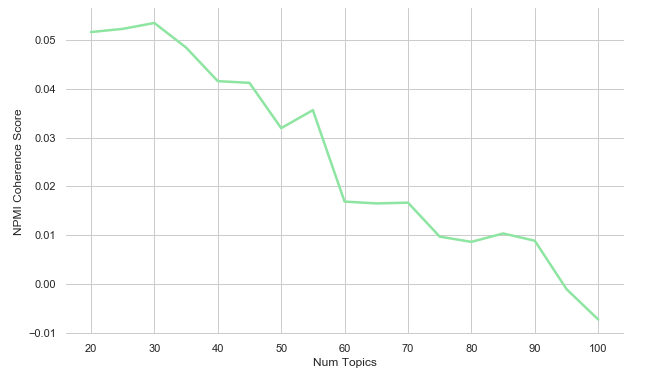
\includegraphics[width=\paperwidth, height=0.4\paperheight, keepaspectratio]{topic_modelling/NPMI_K_Optimo2.PNG}
}
\end{frame}

\begin{frame}
\frametitle{Tópicos descubiertos}
\begin{table}[ht]
\centering
\resizebox{\textwidth}{!}{{\begin{tabular}{|ccll|}
  \hline
 \textbf{Número de topico} & \textbf{Coherence} & \textbf{Palabras} & \textbf{Etiqueta}\\
  \hline
22 & 0.14 & wear, clothe, bathroom, shirt, shoe, dress, toilet, pant, clean, pair & Vestimenta\\
7 & 0.10 & car, run, drive, road, plane, gun, fly, shoot, stop, hit & Accidente\\
15 & 0.10 & play, stage, music, game, show, name, audience, write, piano, singe & Entretenimiento\\
17 & 0.09 & room, door, bed, open, sleep, leave, window, lock, bedroom, find & Dormitorio\\
23 & 0.08 & work, paper, computer, write, picture, different, word, information, page, use & Trabajo\\
20 & 0.08 & car, drive, home, walk, way, road, truck, turn, street, right & Transporte\\
6 & 0.07 & mom, guy, girl, call, stuff, shop, school, place, later, friend & Amigos, escuela, adolescencia\\
4 & 0.07 & water, pool, fire, boat, swim, wave, walk, rock, little, big & Deporte acuático\\
9 & 0.06 & run, tree, horse, jump, fall, dog, big, throw, ball, climb & Deporte al aire libre\\
12 & 0.06 & phone, call, work, photo, office, find, computer, desk, time, number & Oficina\\
5 & 0.06 & class, school, sit, teacher, student, room, next, walk, time, give & Colegio\\
21 & 0.04 & man, walk, woman, hand, kiss, dance, young, old, away, arm & Romance\\
16 & 0.04 & girl, friend, mother, boy, sister, little, house, time, child, dress & Familia\\
24 & 0.04 & kind, really, little, stuff, time, wake, bus, sort, sound, sit & Undefined\\
3 & 0.03 & friend, drink, walk, wedding, eat, bottle, snow, party, dress, find & Fiesta, casamiento\\
18 & 0.03 & die, kill, dead, cry, happen, brother, man, time, leave, feel &  Pérdida, muerte\\
14 & 0.02 & feel, woman, sit, time, man, answer, question, work, room, give & Relaciones interpersonales\\
1 & 0.02 & sit, leave, walk, realize, door, room, stand, table, hand, right & En movimiento\\
0 & 0.02 & work, use, fish, job, test, need, also, different, time, ice & Undefined\\
13 & 0.02 & baby, walk, sit, woman, stand, table, small, find, man, right & Bebes\\
8 & 0.01 & man, light, small, large, group, team, building, long, bird, field & Trabajo\\
11 & 0.01 & leave, feel, mother, find, woman, man, wait, time, help, walk & Relaciones interpersonales\\
19 & 0.01 & train, boy, chicken, tooth, eat, buy, little, money, work, flower & Amigos, escuela, adolescencia\\
10 & 0.01 & room, walk, store, time, woman, man, large, house, building, move &  En movimiento\\
2 & 0.001 & movie, doctor, watch, group, film, episode, nurse, show, woman, move & Películas\\
   \hline
\end{tabular}}}
%\caption{Tópicos descubiertos}
\end{table}
\end{frame}

\subsection{Género y Rango Etario}

\begin{frame}
\frametitle{Distribución de Tópicos por Género}
\begin{columns}
\begin{column}{0.6\textwidth}
Distribución de los sueños de las Mujeres:
\begin{enumerate}
    \item 20\% en \textbf{Amigos/Escuela/ Adolescencia} (6).
    \item 7,5\% en \textbf{Sin definir} (24).
    \item 6\% para \textbf{Relaciones Interpersonales} (14).
\end{enumerate}
\end{column}
\begin{column}{0.4\textwidth}
    \makebox[\textwidth]{
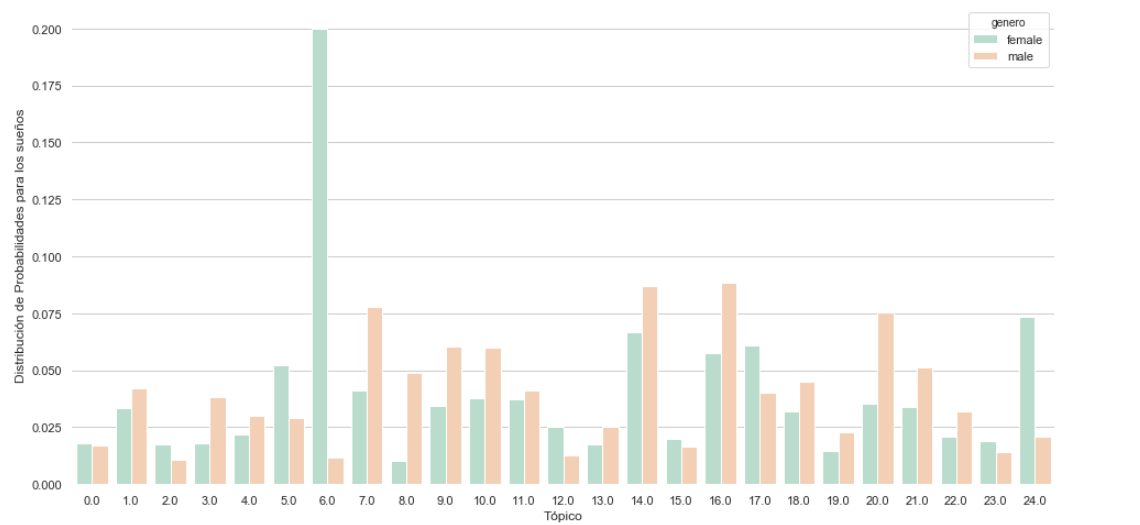
\includegraphics[width=0.5\paperwidth, height=0.7\paperheight, keepaspectratio]{data/topic_modelling/Genero_TopicModelling.png}
}
\end{column}
\end{columns}
\end{frame}

\begin{frame}
\frametitle{Distribución de Tópicos por Género}
\begin{columns}
\begin{column}{0.6\textwidth}
Distribución de los sueños de los Hombres:
\begin{enumerate}
    \item 8-9\% en \textbf{Relaciones Interpersonales} (14) y \textbf{Familia} (16).
    \item 7.5\% en \textbf{Accidente} (7).
\end{enumerate}
\end{column}
\begin{column}{0.4\textwidth}
    \makebox[\textwidth]{
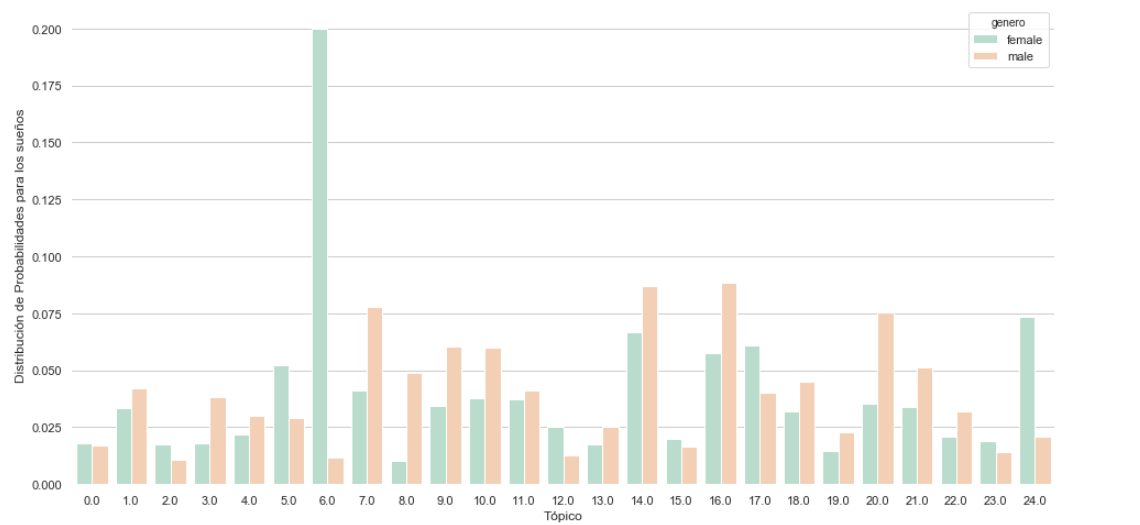
\includegraphics[width=0.5\paperwidth, height=0.7\paperheight, keepaspectratio]{data/topic_modelling/Genero_TopicModelling.png}
}
\end{column}
\end{columns}
\end{frame}

\begin{frame}
\frametitle{Distribución de Tópicos por Rango Etario}
\makebox[\textwidth]{
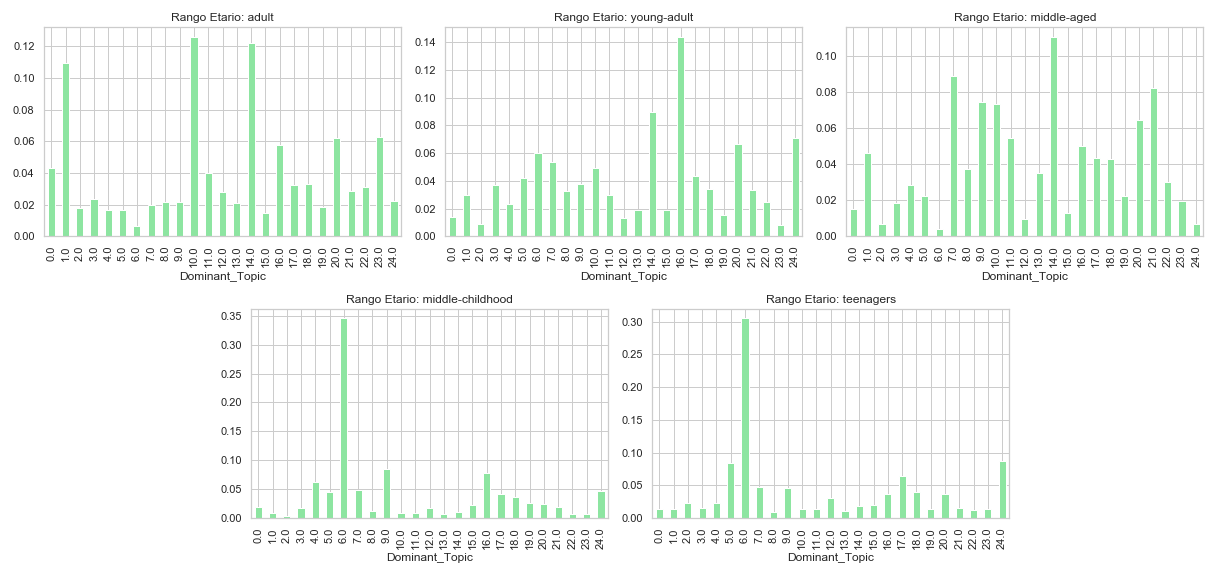
\includegraphics[width=\paperwidth, height=0.6\paperheight, keepaspectratio]{data/topic_modelling/RangoEtario_TopicModelling_3.png}
}

\end{frame}

\begin{frame}
\frametitle{Distribución de Tópicos por Rango Etario}
Se analizaron cerca de 19 mil sueños, ya que se dejaron fuera los sueños etiquetados como series (por pertenecer a diferentes grupos etarios) y los sueños registrados por personas al azar.\\
\end{frame}

\begin{frame}
\frametitle{Distribución de Tópicos por Rango Etario}
\begin{itemize}
\setbeamertemplate{itemize items}[triangle]
        \item \textit{Niños}: Los sueños se distribuyen en un 35\% en el Tópico \textbf{Amigos/Escuela/Adolescencia} (6).
        \item \textit{Adolescentes}: se distribuyen en un 30\% en el Tópico \textbf{Amigos/Escuela/Adolescencia} (6).
        \item \textit{Adulto Joven}: se distribuyen en un 14\% en el Tópico \textbf{Familia} (16).
        \item \textit{Adulto}: se distribuyen en más de un 12\% en el Tópico \textbf{En Movimiento} (10) y en \textbf{Relaciones Interpersonales} 14.
        \item \textit{Adulto Media Edad}: se distribuyen en más de un 10\% en el Tópico \textbf{Relaciones Interpersonales} (14) y en más de un 8\% en \textbf{Accidente} (7).
\end{itemize}
\end{frame}

\subsection{Phil y Vietnam Vet}

\begin{frame}
\frametitle{Cómo sueñan Phil y Vietnam Vet}
\makebox[\textwidth]{
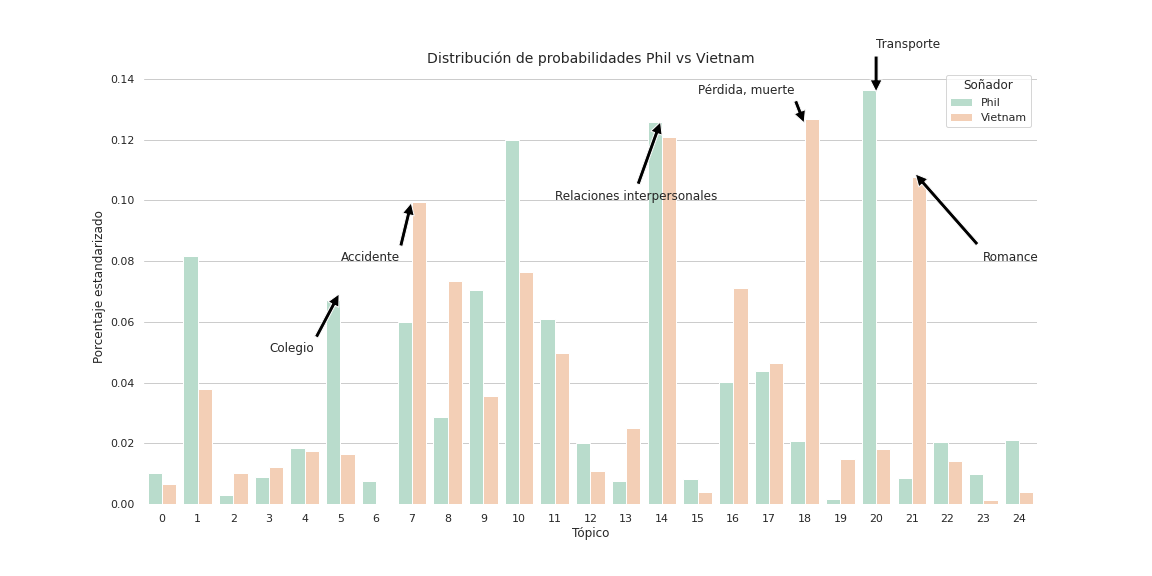
\includegraphics[width=\paperwidth]{topic_modelling/topics_phil_viet.png}
}
\end{frame}

\begin{frame}
\frametitle{Como sueñan Phil y Vietnam Vet}
\begin{itemize}
\setbeamertemplate{itemize items}[triangle]
    \item En los sueños del veterano de Vietnam se puede ver una marcada diferencia en los tópicos relacionados con \textit{Pérdida}, \textit{Accidente} y \textit{Romance}.
    \item En los sueños de Phil se ve una clara predominancia del tópico catalogado como \textit{Transporte} y \textit{Amigos}.
\end{itemize}
    
\end{frame}

\subsubsection{Vietnam Vet}

\begin{frame}
\frametitle{Vietnam Vet y sus etapas}
\makebox[\textwidth]{
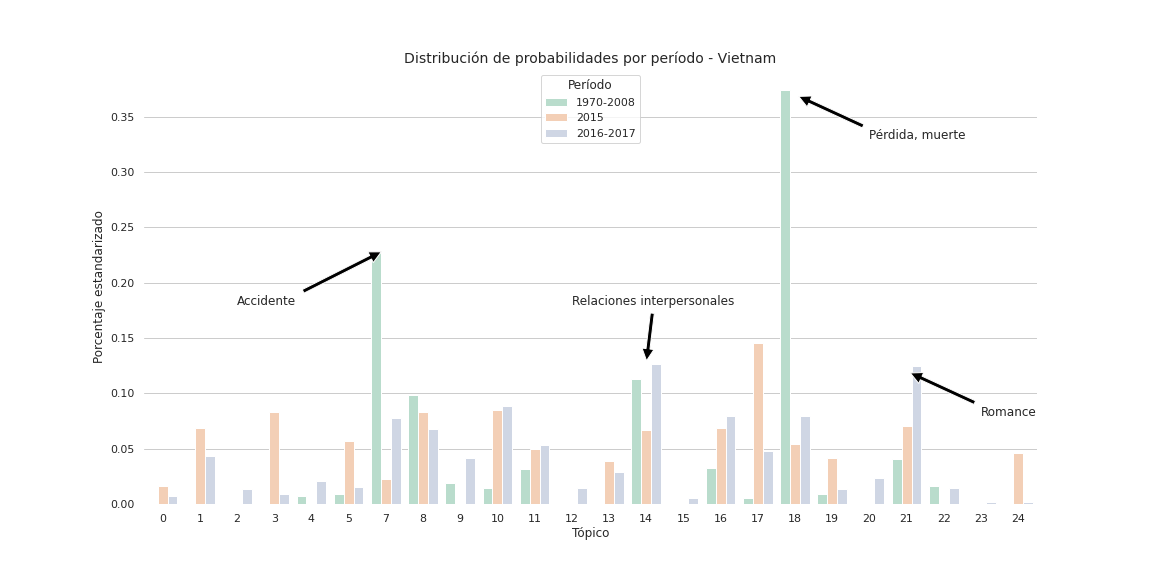
\includegraphics[width=\paperwidth]{topic_modelling/topics_viet_year.png}
}
\end{frame}

\begin{frame}
\frametitle{Vietnam Vet y sus etapas}
\begin{enumerate}
    \item En primer lugar hay que notar que el tópico \textit{Amigos, escuela} tiene probabilidad 0 en las 3 etapas de sueños reportados, y el catalogado como \textit{Colegio} tiene muy baja probabilidad.
    \item Los tópicos de \textit{Accidente} y \textit{Pérdida, muerte} tiene una alta probabilidad en el primer período reportado, para luego en los subsiguientes disminuir notoriamente.
    \item Es interesante ver como el tópico \textit{Romance} incrementa a través de los períodos de forma significativa.
\end{enumerate}
\end{frame}

\subsubsection{Phil}

\begin{frame}
\frametitle{Phil y sus etapas}
\makebox[\textwidth]{
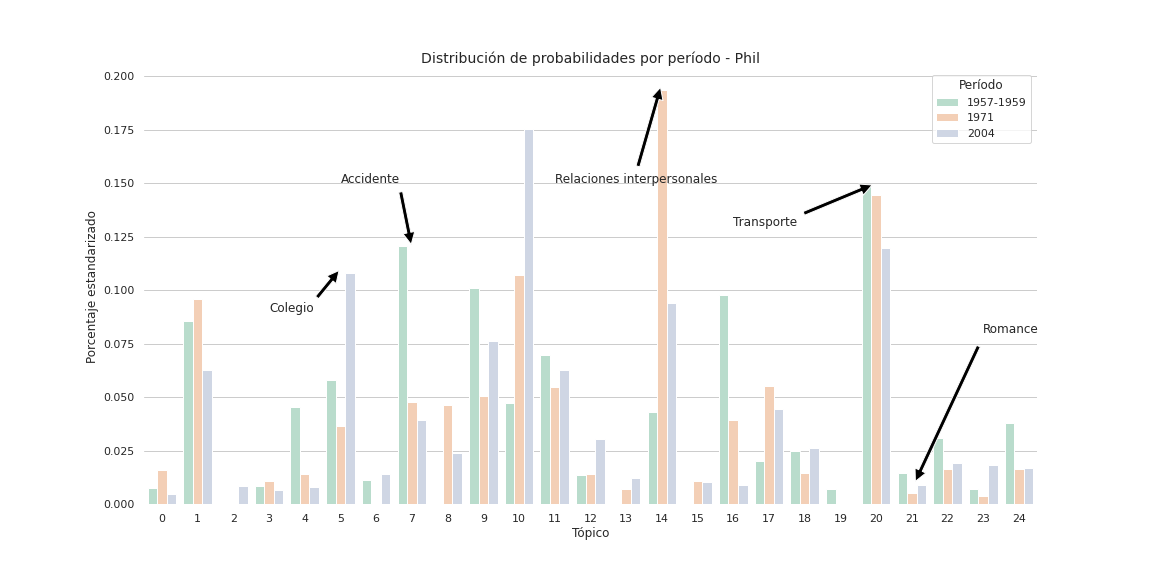
\includegraphics[width=\paperwidth]{topic_modelling/topics_phil_year.png}
}
\end{frame}

\begin{frame}
\frametitle{Phil y sus etapas}
\begin{enumerate}
    \item Se puede observar una alta predominancia del tópico \textit{Relaciones interpersonales} en su primer período de sueños.
    \item El tópico \textit{Transporte} prácticamente no cambia a lo largo del tiempo.
    \item A excepción de algunos pocos tópicos, todos se encuentran con algún porcentaje de participación en los tres períodos reportados.
\end{enumerate}
\end{frame}

\section{Sentiment Analysis}

\subsection{Preprocesamiento y Lexicon}

\begin{frame}
\frametitle{Inducción}
\begin{itemize}
\setbeamertemplate{Lexicon}[triangle]
	\item Pre procesamiento
	\begin{itemize}
	\setbeamertemplate{minusculas}[circle]
		\item Pasar todo el corpus a minúsculas
		\item Eliminar caracteres especiales
	\end{itemize}	
		\begin{columns}
\begin{column}{0.5\textwidth}
    \makebox[\textwidth]{
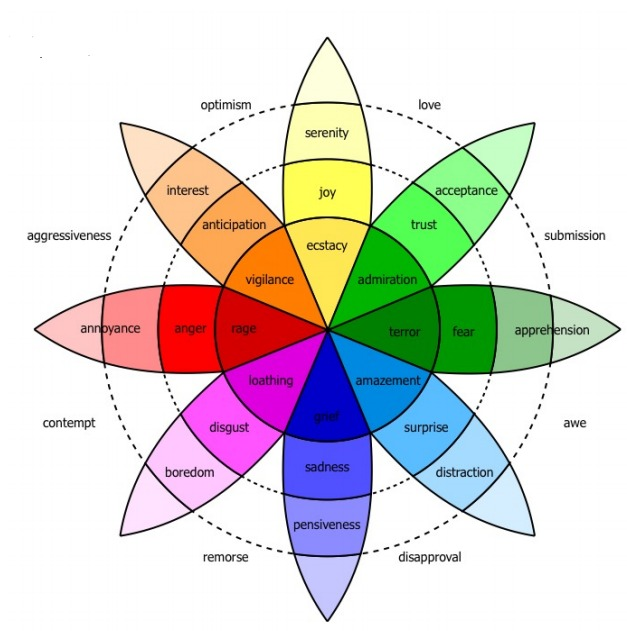
\includegraphics[width=0.6\paperwidth, height=0.5\paperheight, keepaspectratio]{/sa/img/paleta.jpeg}
}
\end{column}
\begin{column}{0.3\textwidth}
\begin{itemize}
    \item Trust
    \item Joy
    \item Fear
    \item Sadness
    \item Anger
    \item Anticipation
    \item Disgust
    \item Surprise
\end{itemize}
\end{column}
\end{columns}
	\end{itemize}
\end{frame}


\begin{frame}
\begin{figure}[h]
\frametitle{Lexicones}
\makebox[\textwidth]{
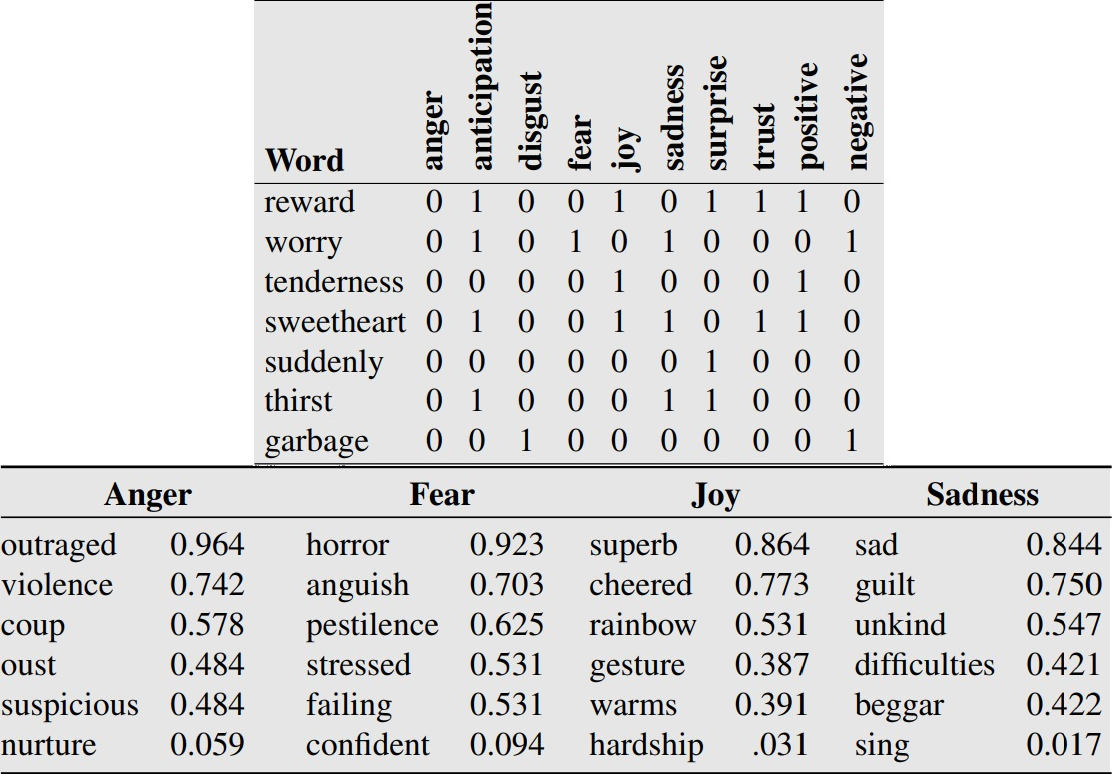
\includegraphics[width=0.55\paperwidth, height=0.6\paperheight, keepaspectratio]{/sa/img/lexicons.png}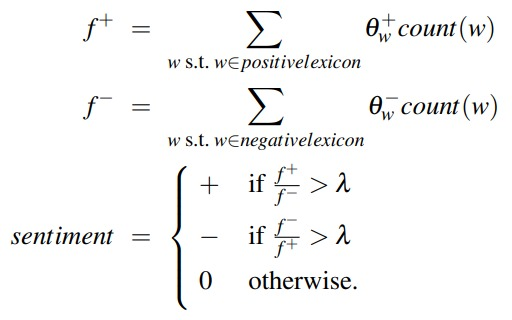
\includegraphics[width=0.4\paperwidth, height=0.6\paperheight, keepaspectratio]{/sa/img/formula.png}
}
\end{figure}
\end{frame}



\subsection{Análisis segmentado}

\begin{frame}
\begin{figure}[h]
\frametitle{Análisis en todo el corpus}
\makebox[\textwidth]{
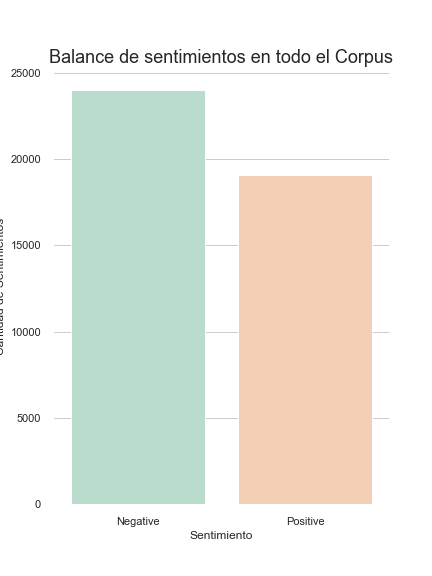
\includegraphics[width=0.4\paperwidth, height=0.6\paperheight, keepaspectratio]{/sa/img/corpus_sentimiento.png}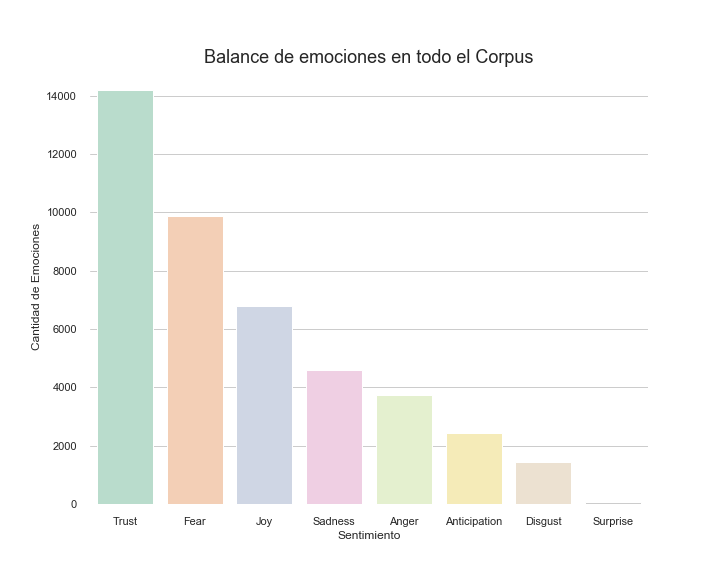
\includegraphics[width=0.6\paperwidth, height=0.6\paperheight, keepaspectratio]{/sa/img/corpus_emocion.png}
}
\end{figure}
\end{frame}


\begin{frame}
\begin{figure}[h]
\frametitle{Análisis por sexo}
\makebox[\textwidth]{
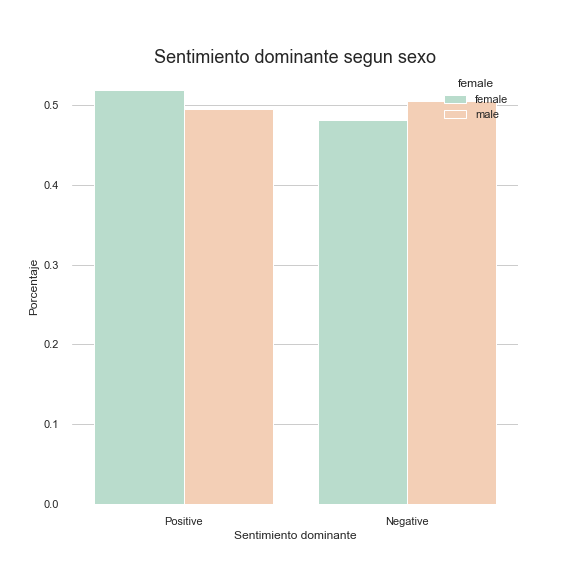
\includegraphics[width=0.4\paperwidth, height=0.6\paperheight, keepaspectratio]{/sa/img/sentimientos_sexos_porcentaje.png}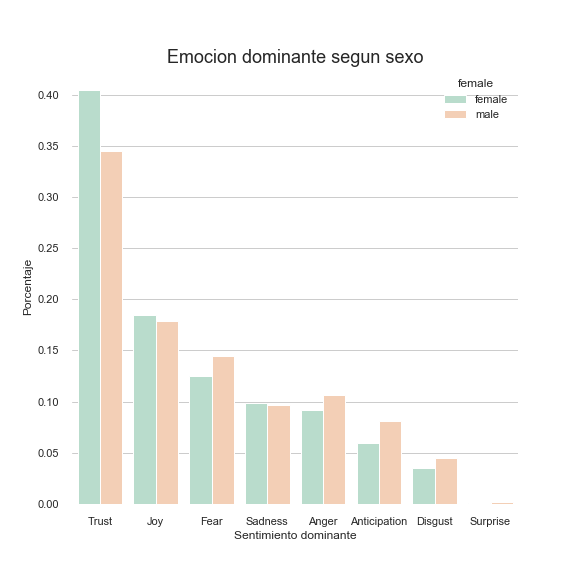
\includegraphics[width=0.6\paperwidth, height=0.6\paperheight, keepaspectratio]{/sa/img/emocion_sexos_porcentaje.png}
}
\end{figure}
\end{frame}


\begin{frame}
\begin{figure}[h]
\frametitle{Análisis por franja etaria}
\makebox[\textwidth]{
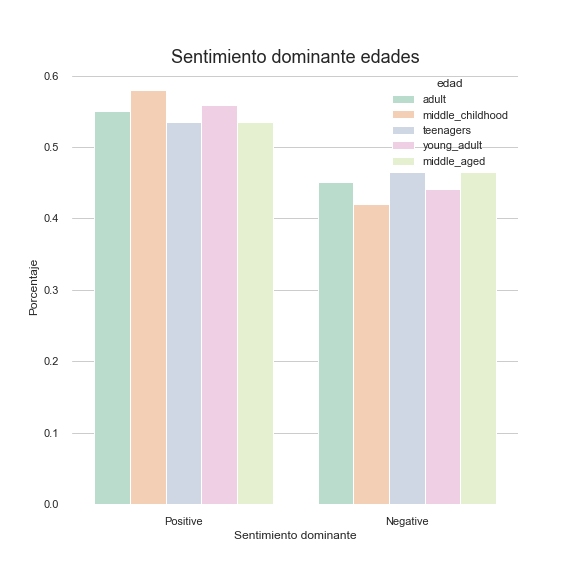
\includegraphics[width=0.4\paperwidth, height=0.5\paperheight, keepaspectratio]{/sa/img/sentimientos_edades_porcentaje.png}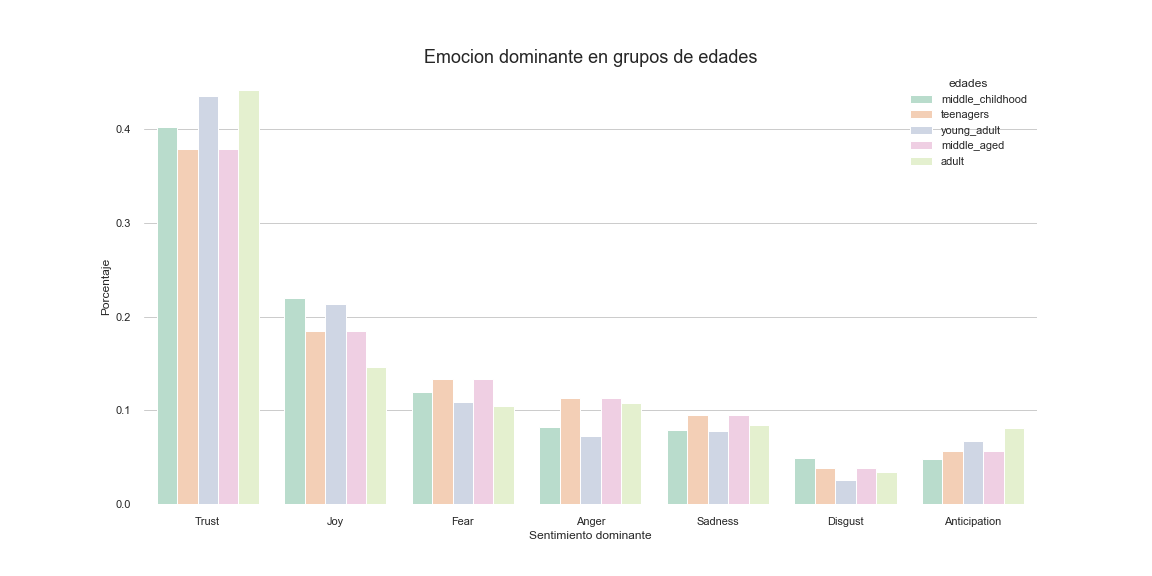
\includegraphics[width=0.6\paperwidth, height=0.6\paperheight, keepaspectratio]{/sa/img/emociones_edades_porcentaje.png}
}
\end{figure}
\end{frame}


\begin{frame}
\begin{figure}[h]
\frametitle{Análisis Phil y Vietnam Vet}
\makebox[\textwidth]{
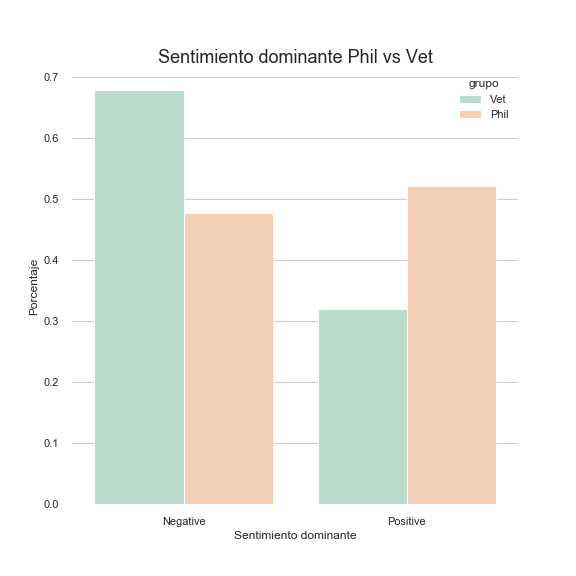
\includegraphics[width=0.4\paperwidth, height=0.6\paperheight, keepaspectratio]{/sa/img/sentimiento_grupo_porcentaje.png}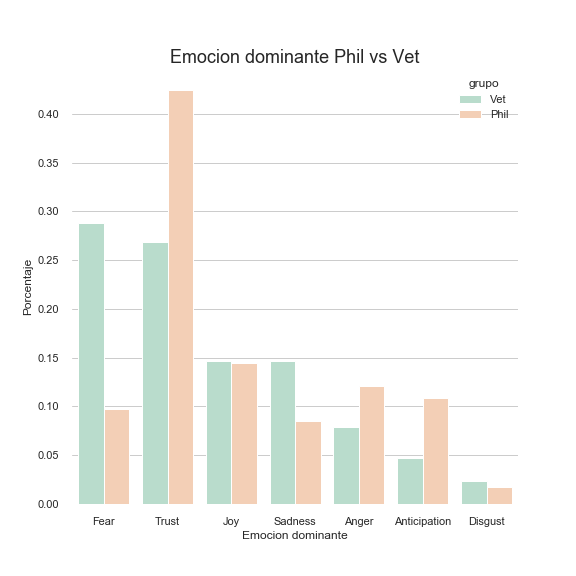
\includegraphics[width=0.6\paperwidth, height=0.6\paperheight, keepaspectratio]{/sa/img/emociones_grupo_porcentaje.png}
}
\end{figure}
\end{frame}

\subsection{Evolución}

\begin{frame}
\begin{figure}[h]
\frametitle{Evolución de emociones en el tiempo Phil y Vietnam Vet}
\makebox[\textwidth]{
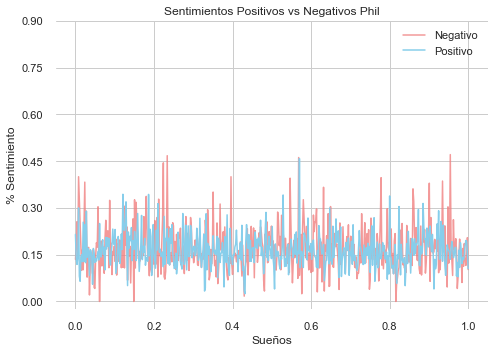
\includegraphics[width=0.45\paperwidth, height=0.45\paperheight, keepaspectratio]{/sa/img/pos_vs_neg_phil.png}
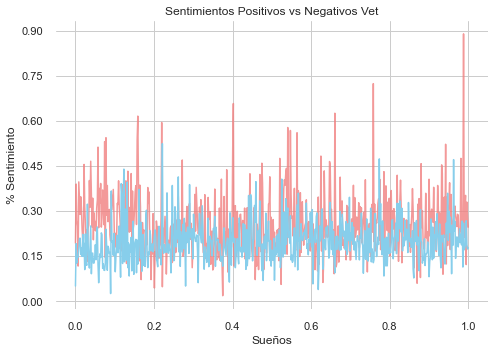
\includegraphics[width=0.45\paperwidth, height=0.45\paperheight, keepaspectratio]{/sa/img/pos_vs_neg_vet.png}
}
\end{figure}
\end{frame}

\begin{frame}
\begin{figure}[h]
\frametitle{Evolución de emociones en el tiempo Phil y Vietnam Vet}
\begin{center}
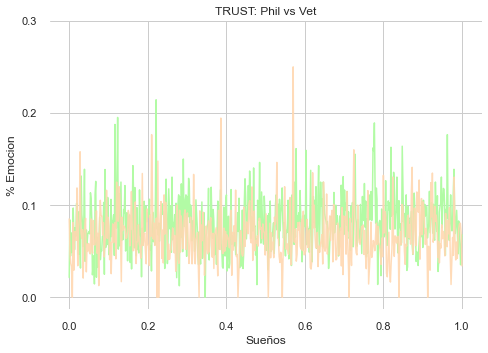
\includegraphics[width=.4\textwidth]{/sa/img/trust_phil_vs_vet.png}
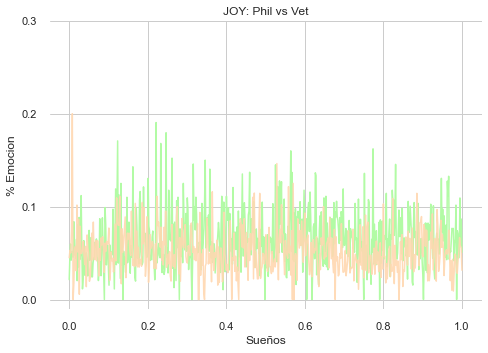
\includegraphics[width=.4\textwidth]{/sa/img/joy_phil_vs_vet.png}
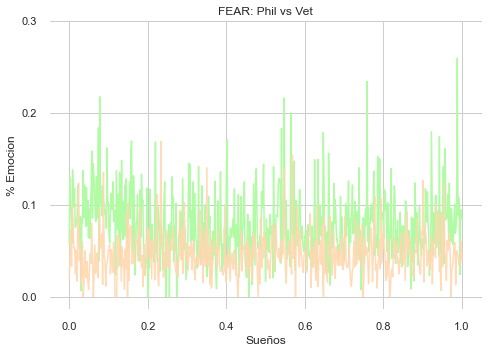
\includegraphics[width=.4\textwidth]{/sa/img/fear_phil_vs_vet.png}
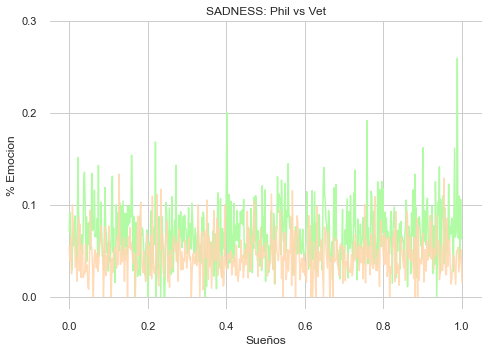
\includegraphics[width=.4\textwidth]{/sa/img/sadness_phil_vs_vet.png}
\end{center}
\end{figure}
\end{frame}



\section{Word Embeddings}

\subsection{Procesamiento}

\begin{frame}
\frametitle{Pasos de Procesamiento}
\resizebox{0.8\paperwidth}{0.5\paperheight}{
\begin{tikzpicture}[node distance=1.5cm,
    every node/.style={fill=white, font=\sffamily}, align=center]
  % Specification of nodes (position, etc.)
  \node (start) [activityRuns] {Corpus completo};
  \node (cleanStep) [process, below of=start, yshift=-0.4cm] {PreProcesamiento};
  \node (w2vStep) [process, right of=cleanStep, xshift=3cm] {Word2Vec};
  \node (weStep) [process, right of=w2vStep, fill=red!30, xshift=3cm] {Word Embeddings};
 
  \node (wepvStep) [process, below of=weStep, yshift=-0.4cm] {Filtro  PHIL y VET};
  \node (DocvStep) [process, left of=wepvStep, xshift=-3cm] {Document Vector};
  \node (ClusStep) [process, left of=DocvStep, xshift=-3cm] {Clustering};
   \node (EtiqStep) [process, left of=ClusStep, xshift=-3cm] {Etiquetado manual};
  \node (finalStep) [startstop, below of=EtiqStep, yshift=-0.4cm] {Clusters etiquetados};
   
 % \node (bigramStep) [process, right of=tokenStep, xshift=4cm] %{Generación de Bi-gramas};
 % \node (lemmaStep) [process, below of=bigramStep, yshift=-0.5cm] %{Lematización};
 % \node (tdfStep) [process, left of=lemmaStep, xshift=-4cm] %{TermDocumentFrequency};
 % \node (finalStep) [startstop, below of=tdfStep, yshift=-0.5cm] %{Diccionario final};
 
  % Specification of lines between nodes specified above
  % with aditional nodes for description 
  %\draw[->] (start) -- (cleanStep);
  \draw[->] (start) -- (cleanStep);
  \draw[->] (cleanStep) node[text width=3.1cm, xshift=3cm, yshift=-0.8cm] {36202 sueños} --  (w2vStep);
  \draw[->] (w2vStep) --  (weStep);
  \draw[->] (weStep) --  (wepvStep);
    \draw[->] (wepvStep) node[text width=3.1cm, xshift=-2cm, yshift=-1cm] {506 y 593 sueños} -- (DocvStep);
  \draw[->] (DocvStep) --  (ClusStep);
  \draw[->] (ClusStep) node[text width=3.1cm, xshift=-2cm, yshift=-0.9cm] {5 y 8 clusters}--  (EtiqStep);
  \draw[->] (EtiqStep) --  (finalStep);
  
  
  \end{tikzpicture}}
\end{frame}

\begin{frame}
\frametitle{Word Embedding y Clustering}
Se ejecutó Word2Vec sobre todo el corpus y se calculó el vector promedio por cada sueño de Phil y Vet.
\begin{itemize}
\setbeamertemplate{itemize items}[triangle]
	\item<1-> Word2Vec con dim=20, window=10, y skipgram
\end{itemize}

\setlength{\parskip}{2em}
Sobre los vectores promedios se hizo clustering para agrupar los sueños por similaridad semántica.
\setlength{\parskip}{0em}
\begin{itemize}
\setbeamertemplate{itemize items}[triangle]
	\item<1-> Clusterización con método jerárquico y kmeans
	\item<1-> Validación de los clusters con coeficiente de Silhouette
\end{itemize}
\end{frame}

\begin{frame}
\frametitle{Clusters obtenidos}
\renewcommand{\arraystretch}{1.5}
\begin{table}[ht]
\centering
\resizebox{\textwidth}{!}{{\begin{tabular}{|cl|}
\multicolumn{2}{c}{SERIES VET} \\
\hline
\textbf{Etiqueta Manual} & \textbf{Palabras que se destacan}\\
\hline
"casa/hotel" & home - kitchen -room – bedroom - hotelroom -bed -house -toilet -furnished - door \\
"guerra" & bomb  - fear - pain - dying  - frightened - war - escape  run - blood - afraid - explode\\
"familia/amigos" & girlfriend - fríend  - dinner - mother - family - brother – veterans - dog \\
"huir" & prison -  escape -  climb - speed - far away - run – hide - accelerate\\
"guerra" & fear  - death - killing - attack - shoot - kick -  struggle - fight - shoot - soldier \\
"mujeres" & woman – attractive - massage - love - girl - feel good - beautiful\\
"clases/hospital" & medic -  class - clinic - students -  hospital - teacher- write - tell - psychologist\\
"miscelaneous" & college - theater - moving - changes - wearing - game - cloth - team\\
\hline
\end{tabular}}}
%\caption{Clusters}
\end{table}
\end{frame}

\begin{frame}
\frametitle{Clusters obtenidos}
\renewcommand{\arraystretch}{1.5}
\begin{table}[ht]
\centering
\resizebox{\textwidth}{!}{{\begin{tabular}{|cl|}
\multicolumn{2}{c}{SERIES PHIL} \\
\hline
\textbf{Etiqueta Manual} & \textbf{Palabras que se destacan}\\
\hline
"clases/teaching" & classes - school - univesity - collegue - job - office - work - friends - semester \\
"campo/exterior" & river - car - boats  - bridge - swim - water - mountain - farm - trees - walking - falling\\
"mujeres" & relation - kiss - sex - blood - naked\\
"deportes" & games - football - basketball - handball - league- team\\
"familia/amigos" & trip - house - home - car - family - wife - drive - bus - leave - go - meeting\\
\hline
\end{tabular}}}
%\caption{Clusters}
\end{table}
\end{frame}

\begin{frame}
\frametitle{Clusters obtenidos}
Validación por Silhouette
\makebox[\textwidth]{
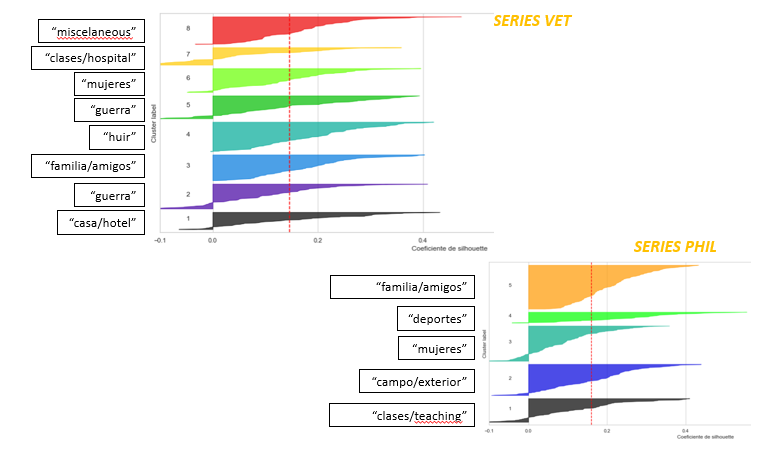
\includegraphics[width=\paperwidth, height=0.6\paperheight, keepaspectratio]{we/validacion_clusters.PNG}
}
\end{frame}

\subsection{Análisis Series Phil y Vet}

\begin{frame}
\begin{figure}[h]
\frametitle{Distribución de las series en los clusters}
\begin{center}
  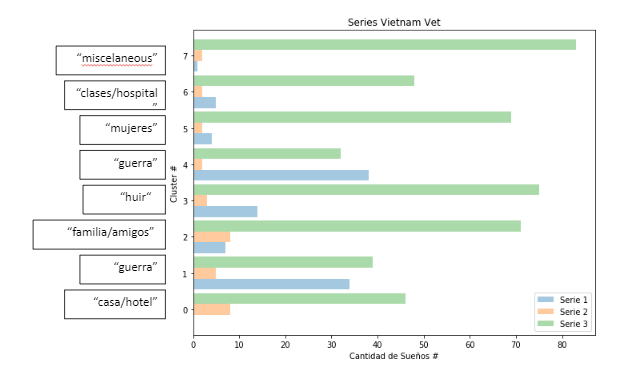
\includegraphics[width=0.45\textwidth, keepaspectratio]{we/vet_series_bars.PNG}
  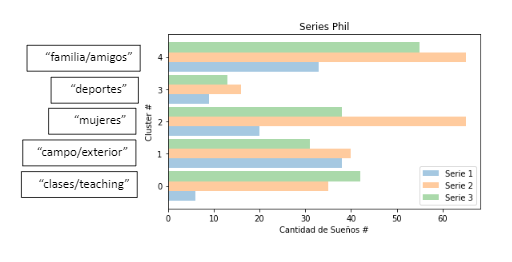
\includegraphics[width=0.45\textwidth, keepaspectratio]{we/phil_series_bars.PNG}
  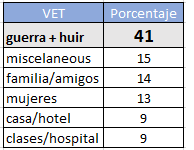
\includegraphics[width=0.2\textwidth]{we/vet_resumen.PNG}
  \hspace{5em}
  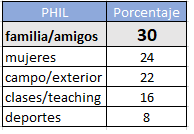
\includegraphics[width=0.2\textwidth]{we/phil_resumen.PNG}
\end{center}
\end{figure}
\end{frame}

\begin{frame}
\frametitle{Recurrencia de sueños}
Sueños de Vet en distintas etapas de la vida
\makebox[\textwidth]{
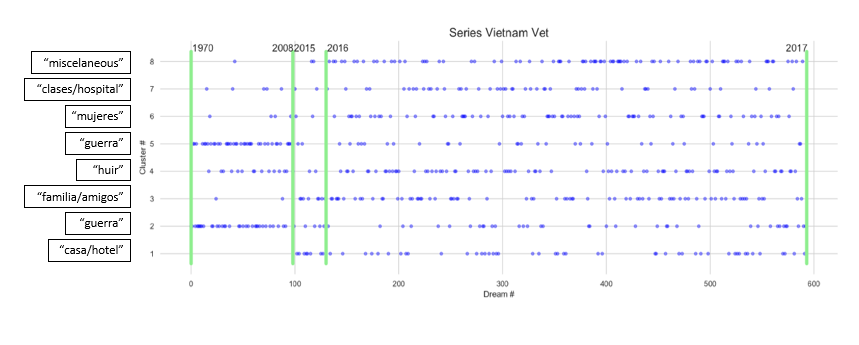
\includegraphics[width=\paperwidth, height=\paperheight, keepaspectratio]{we/vet_series_clusters.PNG}
}
\end{frame}

\begin{frame}
\frametitle{Recurrencia de sueños}
Sueños de Phil en distintas etapas de la vida
\makebox[\textwidth]{
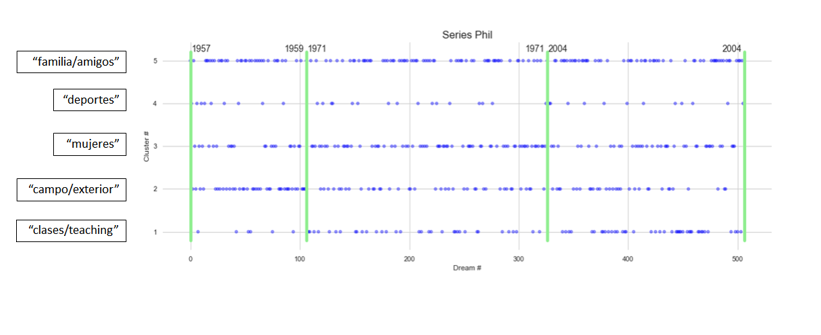
\includegraphics[width=\paperwidth, height=\paperheight, keepaspectratio]{we/phil_series_clusters.PNG}
}
\end{frame}


\begin{frame}
\frametitle{La recurrencia en números}
Medida como la cantidad de veces que se repite un cluster en ventana de 10 sueños consecutivos
\makebox[\textwidth]{
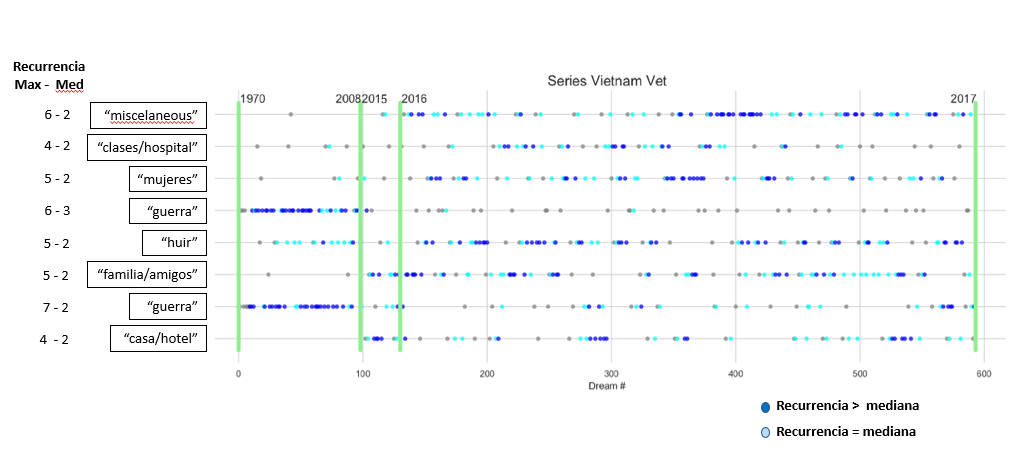
\includegraphics[width=\paperwidth, height=\paperheight, keepaspectratio]{we/vet_recurrencia.PNG}
}
\end{frame}

\begin{frame}
\frametitle{La recurrencia en números}
Calculado con la función rolling() de Pandas
\makebox[\textwidth]{
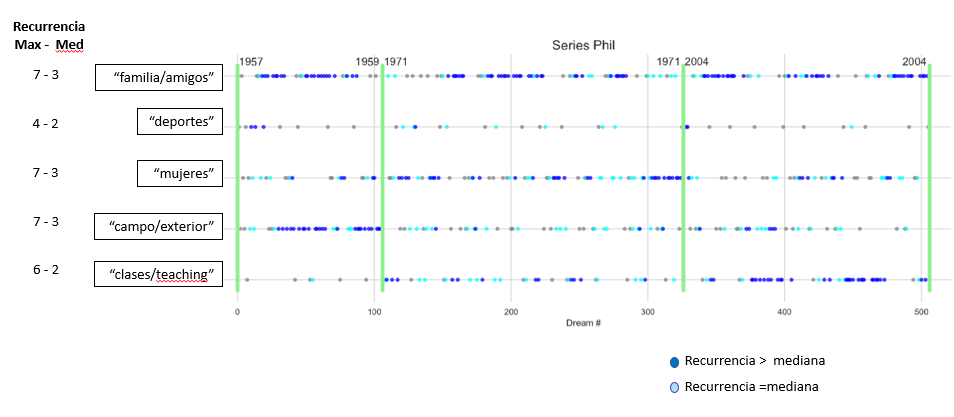
\includegraphics[width=\paperwidth, height=\paperheight, keepaspectratio]{we/phil_recurrencia.PNG}
}
\end{frame}

\subsection{Compración con Sentiment Analysis y Topic Modeling}
\begin{frame}
\frametitle{Clustering vs Sentiment Analysis}
Sueños de Vet
\makebox[\textwidth]{
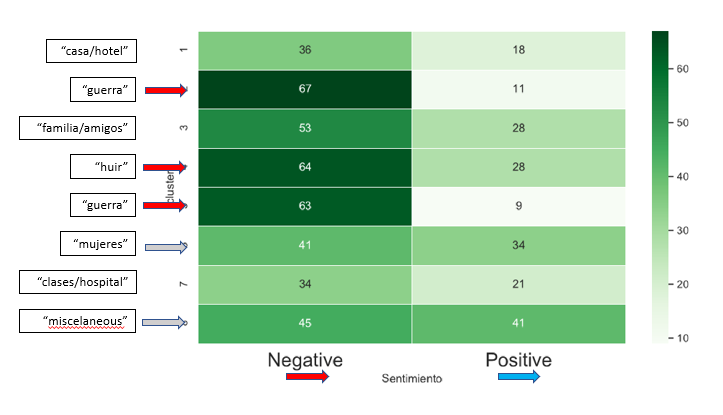
\includegraphics[width=0.8\paperwidth, height=0.8\paperheight, keepaspectratio]{we/vet_clusters_sent.PNG}
}
\end{frame}


\begin{frame}
\frametitle{Clustering vs Sentiment Analysis}
Sueños de Phil
\makebox[\textwidth]{
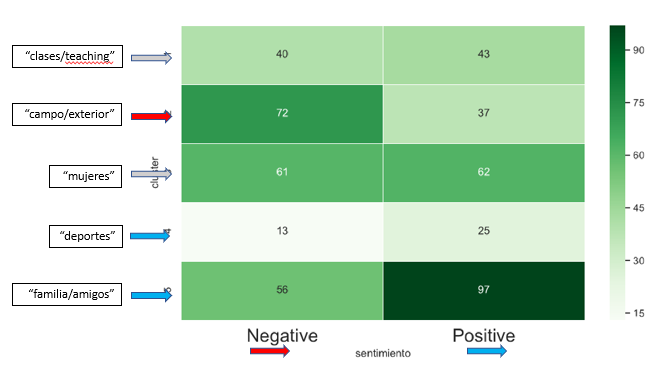
\includegraphics[width=0.8\paperwidth, height=0.8\paperheight, keepaspectratio]{we/phil_clusters_sent.PNG}
}
\end{frame}


\begin{frame}
\frametitle{Clustering vs Topic Modelling}
Sueños de Vet
\makebox[\textwidth]{
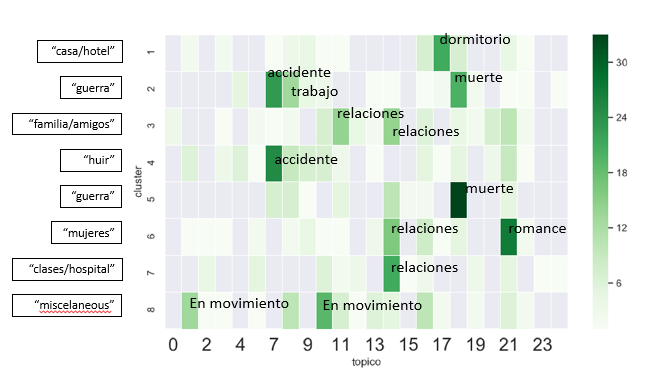
\includegraphics[width=0.8\paperwidth, height=0.8\paperheight, keepaspectratio]{we/vet_clusters_topico.PNG}
}
\end{frame}


\begin{frame}
\frametitle{Clustering vs Topic Modelling}
Sueños de Phil
\makebox[\textwidth]{
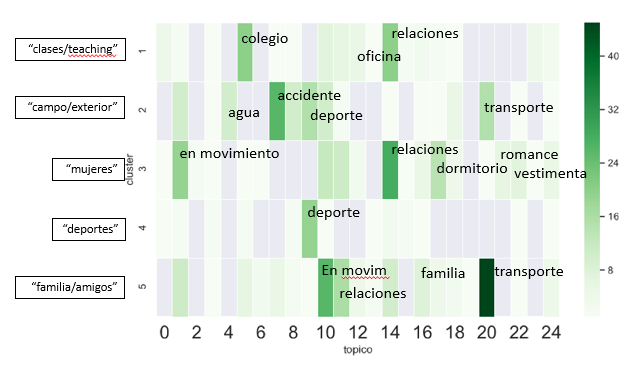
\includegraphics[width=0.8\paperwidth, height=0.8\paperheight, keepaspectratio]{we/phil_clusters_topico.PNG}
}
\end{frame}

\section{Conclusiones}
\begin{frame}
\frametitle{Conclusiones}
Se confirmaron las diferencias entre Phil y Vet. Phil tiene una distribución uniforme de los temas de los sueños siendo los principales temas de familia, amigos, trabajo, vida cotidiana (sentimientos positivos). Mientras que Vet tiene mayoría cercana al 41\% de sueños relacionados con la guerra y pesadillas de persecución(sentimientos negativos), y recurrentes en las tres series.\\
En cuanto a los sueños de los distintos grupos de edades no se encontraron diferencias en las emociones reportadas y los temas encontrados para cada uno fueron los esperados.
\end{frame}

\begin{frame}
\frametitle{Preguntas}
\makebox[\textwidth]{

\includegraphics[width=0.7\paperwidth, height=0.6\paperheight, keepaspectratio]{preg1.png}
}
\end{frame}

\end{document}
